\chapter{The Myo Armband}
\label{chap:myo}
This report is based on the use of the Myo armband, and this chapter will cover a brief description of the Myo device, such as hardware specification and software functionality. The Myo armband, developed by Thalmic Labs, is a wearable gesture and motion control device that uses a set of electromyographic (EMG) sensors that sense electrical activity, combined with an Inertial Measurement Unit (IMU) including gyroscope, accelerometer and magnetometer, to recognize gestures \cite{myo}.

\begin{figure}[ht]
    \centering
    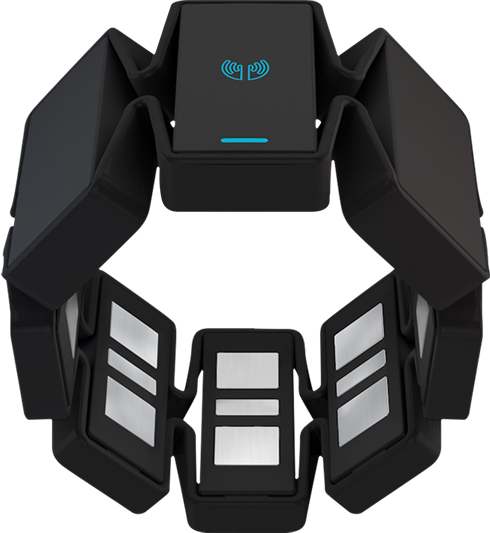
\includegraphics[height=5cm]{content/03-Myo_Armband/images/myo.png}
    \captionsource{\url{https://static.thalmic.com/sapphire/tenFootExperience/hero/myo.png}}
    \caption[The Myo Armband]{The Myo Armband}
    \label{fig:myoarmband}
\end{figure}


\section{Hardware}
The Myo armband consist of eight EMG sensors and nine-axis IMU containing gyroscope, accelerometer and magnetometer. The hardware specification is shown in \cref{table:myo_hardware}.

\begin{table}[ht!]
\centering
    \begin{tabular}{ | l | p{8cm} |}
        \hline
        \textbf{Sensors} & EMG sensor,\newline Gyroscope,\newline Accelerometer, \newline Magnetometer\\ \hline
        
        \textbf{Processor} & ARM Cortex M4 Processor  \\ \hline
        
        \textbf{Feedback} & Dual Indicator LEDs,\newline Short, Medium, Long Vibrations  \\ \hline
    \end{tabular}
    \caption[The Myo Hardware]{List of The Myo Hardware specifications}
    \label{table:myo_hardware}
\end{table}

\section{The Myo SDK}
\label{sec:myoSDK}
Thalmic Labs provides a SDK that allows developers to obtain access to the data from the Myo device. Since the Windows SDK was used, every statements in this report will be based on the Windows SDK. The library at the core of the Myo SDK allows applications to interact with the Myo armband. All functionality in libmyo is exposed through a plain C API. Typically, applications do not interact with the libmyo C API directly. Instead they use a language binding corresponding to the programming language used by the application \cite{myoSDK}.

\Cref{fig:myoSDKstack} illustrates the Myo development stack from an application using the SDK down to a physical Myo device

\begin{figure}[ht]
    \centering
    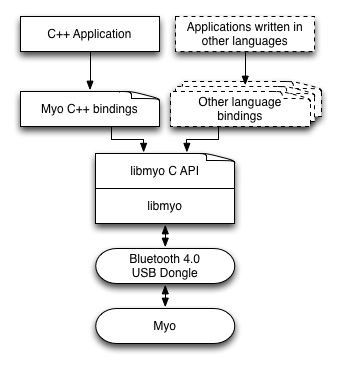
\includegraphics[height=9.5cm]{images/myo-sdk-stack.png}
    \captionsource{\url{https://developer.thalmic.com/docs/api_reference/platform/the-sdk.html}}
    \caption[The Myo SDK stack]{The Myo SDK stack: Myo development stack from an application using the SDK down to a physical Myo device}
    \label{fig:myoSDKstack}
\end{figure}

The Myo armband provide applications with two type of data: Spatial data and gestural data.

\subsection{Spatial Data (IMU)}
Spatial data represents the location of the armband, and informs the applications about orientation and movements. This data is provided by the IMU. The Myo armband output three different data from the IMU: 
\begin{itemize}
  \item raw Accelerometer data
  \item raw Gyroscope data
  \item Orientation data
\end{itemize}
All of the IMU-sensor have a sampling rate of 50 hz. Accelerometer data and gyroscope data is represented as 3D-vectors, with the unit g-force (accelerometer) and deg/s (gyroscope), while the orientation data from the magnetometer is represented as quaternions.

\subsection{Gestural Data (EMG sensor)}
\label{subsec:myoEmgSensor}
Gestural data provide applications with information of less orientation depended movements, such as hand gestures. This data is provided by the EMG sensors. The Myo armband have eight EMG sensors, which outputs raw EMG data of 8-bit with a sampling rate of 200 Hz \footnote{\url{http://developerblog.myo.com/raw-uncut-drops-today/}}. The MyoSDK documentation \cite{myoSDK} does not provide information about the measurement unit for the EMG-data, but the values are converted into a 8-bit value ranging from -128 to 128.